\chapter{Applicatie server - Glassfish}
Een van de applicatie servers die gebruikt worden bij het ontwikkelen van de applicatie is Glassfish. In onderstaande hoofdstukken wordt uitgelegd hoe Glassfish geconfigureerd is in Docker en welke configuratie is toegepast in Glassfish zelf.

\section{Container Configuratie}
Voor het configureren van Glassfish binnen docker maken we gebruik van de laatste versie van Glassfish die beschikbaar is op Docker hub. Op het moment van schrijven is de huidige versie voor Glassfish versie 5.0.

\begin{figure}[H]
	\centering
	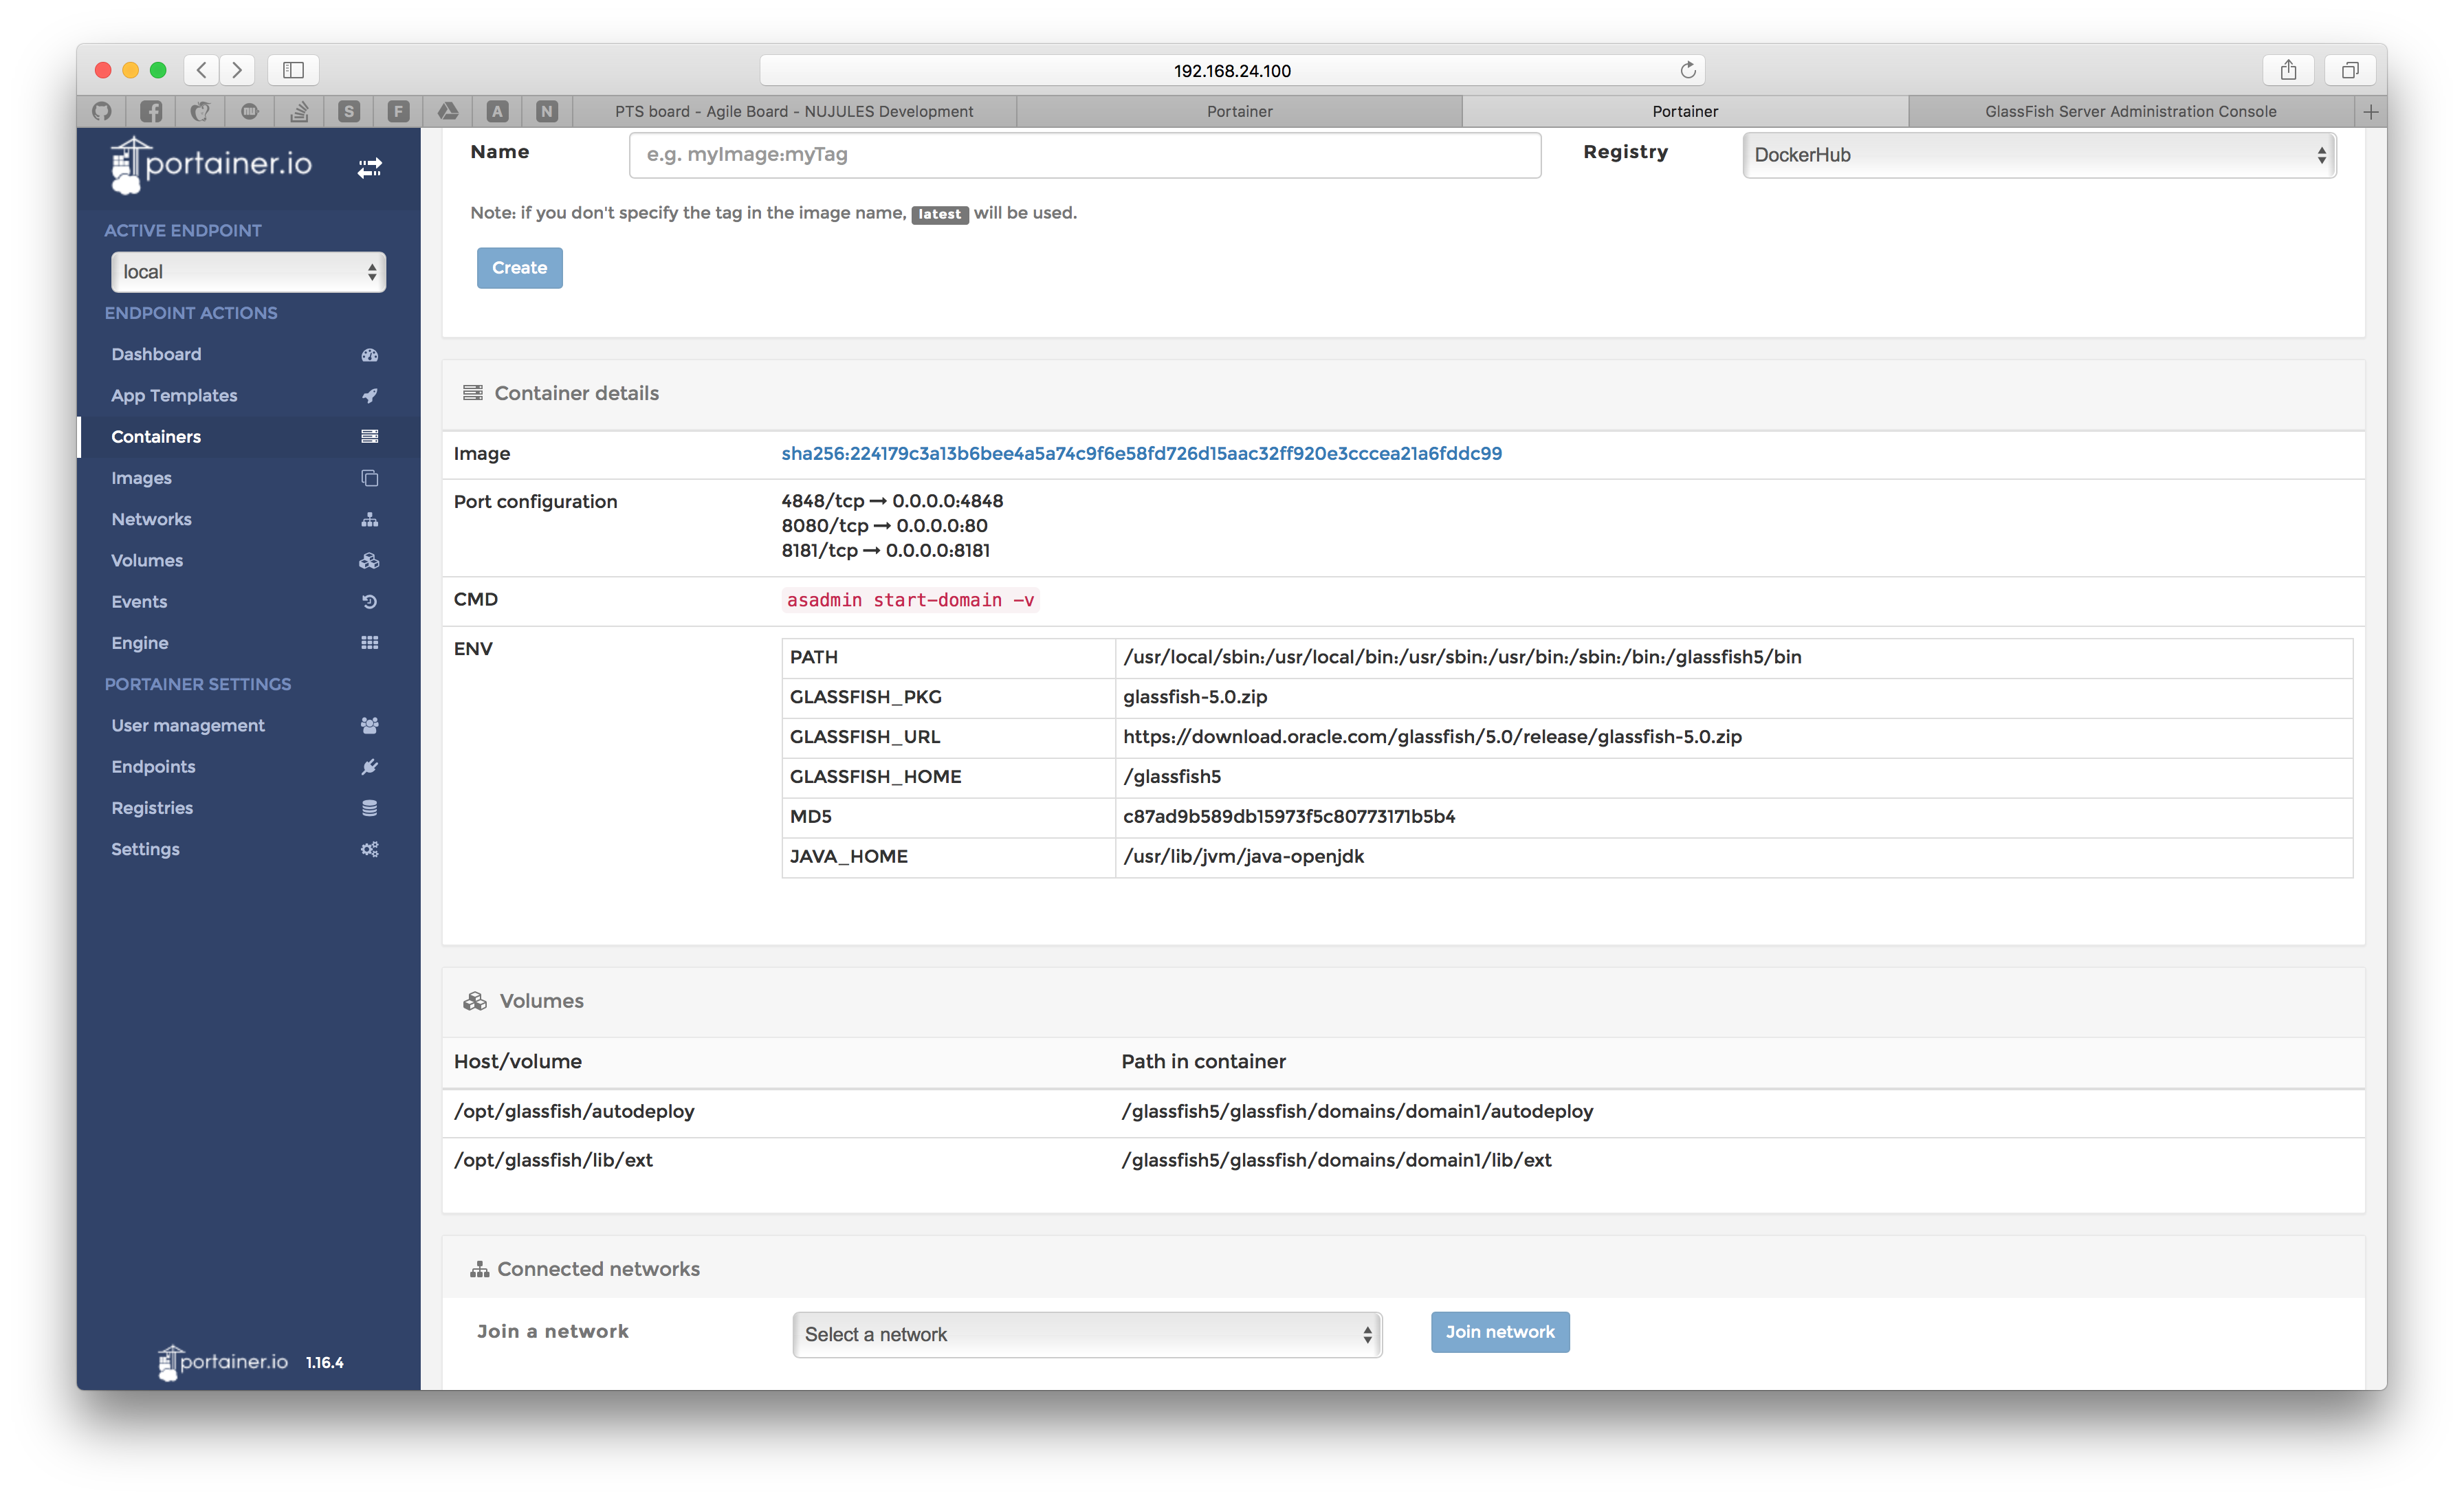
\includegraphics[width=0.95\textwidth]{img/GlassfishConfiguration.png}
	\caption{Configuratie van Glassfish binnen Docker}
	\label{fig:GlassfishConfiguration}
\end{figure}

\subsection{Port mapping}
Zoals we in FIguur \ref{fig:GlassfishConfiguration} kunnen zien, zijn er drie poorten gemapped met de container die communicatie van buiten de container mogelijk maken.

\subsubsection{Poort 4848}
Poort 4848 wordt gebruikt om toegang te krijgen tot de Admin console van glassfish. Het bijbehorend wachtwoord om in te kunnen loggen, is automatisch gegenereerd wanneer Glassfish wordt gestart. Dit wachtwoord kunnen we tevens terug halen door de gegenereerde logs in Portainer te raadplegen.
\newpage
\subsubsection{Poort 8080}
Poort 8080 wordt door Glassfish gebruikt voor HTTP verkeer. Echter hebben we voor deze poort een andere binding moeten opzetten. We hebben ervoor gekozen om dit op poort 80 te doen. Dit wilt dus zeggen dat HTTP verkeer contact kan maken met de Glassfish container via IP adres 192.168.24.100:80.
\newline
De reden dat we een andere poort gebruiken dan standaard poort 8080 is dat de Jenkins instantie reeds op poort 8080 toegankelijk is en deze poort dus niet nogmaals gebruikt kan worden.

\subsubsection{Poort 8181}
Poort 8181 wordt gebruikt voor HTTPS verkeer naar Glassfish. 

\subsection{Volumes}
Aan de hand van Figuur \ref{fig:GlassfishConfiguration} kunnen we zien dat er twee volumes gemapped zijn met de host machine.

\subsubsection{Volume mapping /opt/glassfish/autodeploy}
In Figuur \ref{fig:JenkinsContainerDetails} kunnen we zien dat de Jenkins container ook een binding heeft met de map \begin{lstlisting}
/opt/glassfish/autodeploy
\end{lstlisting}
Omdat we vanuit Jenkins na het bouwen de applicatie kopieren naar de hierboven genoemde map, is de applicatie automatisch beschikbaar binnen de Glassfish container.
\newline
In Figuur \ref{fig:GlassfishConfiguration} zien we het volledige pad waarmee Glassfish gemapped is binnen de container het autodeploy pad is voor Glassfish. Wanneer Jenkins het bouwen van de applicatie afgerond heeft, zals Glassfish automatisch de applicatie proberen te deployen. 
\newline
Natuurlijk is dit enkel van toepassing op de Development omgeving van de applicaties aangezien het deployen van de applicaties naar de Production omgeving handmatig gedaan wordt.
\subsubsection{Volume mapping /opt/glassfish/lib/ext}
Soms kan het voorkomen dat Glassfish voor een correcte werking extra hulpmiddelen/drivers nodig heeft. Denk hierbij bijvoorbeeld aan een database drive om connectie met een database te kunnen maken.
\newline
Vanuit de host machine hebben we door de opgezette mapping binnen de Glassfish Container toegang tot de map waar eventuele benodigde drivers in geplaatst kunnen worden. Hierdoor is het voor ons mogelijk om op een makkelijke manier een nieuwe driver toe te voegen aan Glassfish
\newpage
\subsection{Optimalisatie}
Voor het automatisch deployen van de applicaties op dezelfde server, kunnen we bovenstaande configuratie van Docker gebruiken, echter is dit niet meer van toepassing wanneer we de applicatie op een andere server willen deployen.
\newline
Dit probleem kunnen we oplossen met de Jenkins pluging "Deploy to Container". Hierin kunnen we de gegevens van een Glassfish container opgeven waar de applicatie in gedeployed moet worden.
\newline
\par
Tevens is er een mapping toegepast voor eventuele drivers die nodig zijn bij het deployen van de applicatie. Deze drivers moeten nu handmatig toegevoegd worden aan Glassfish vanuit de host machine. Wanneer de Glassfish container verwijderd wordt, dienen de benodigde drivers opnieuw toegevoegd te worden.\newline
Dit kunnen we oplossen door een eigen Docker Image te maken van de Glassfish image waarin we de benodigde drivers naar de image kopieren.
